\section{Sequences of Fair Coin Flips}\label{sec:1}
Suppose we flip a fair coin p times and record $f_1$ through $f_p$. 
If the coin lands heads on the $j$-th flip,  $f_j = 1$
and if it lands tails, $f_j=0$. Each sequence of $p$ flips will be interpreted 
as a binary number with fixed precision of $p$ digits, 
\begin{equation}
    n_p(\vec f) = 0.f_1f_2\dots f_p = \sum_{j=1}^p \frac{f_j}{2^j}.
    \label{fig:coinflip_sequence}
\end{equation}
Since $f_k$ can only be 1 or 0, it is easy to see that 
$$\min\{n_p(\vec f)\} = 0$$
and 
$$\max\{n_p(\vec f)\} = \sum_{j=1}^p \frac{1}{2^j}.$$
For $p=16$ we get 
\[
    \max\{n_{16}(\vec f)\} = \frac{\num{65535}}{\num{65536}}.
\]
For the special case where $p\rightarrow\infty$ we can rewrite the sequence,
\[
    \max\{n_\infty(\vec f)\} = \sum_{j=1}^\infty \frac{1}{2^j}
    = \sum_{j=0}^\infty \frac{1}{2^j} - 1 = g\qty(\frac{1}{2}) - 1 = 1
\]
where $g(x)$ is the geometric series with the known limit $1 / (1 - x)$ for $|x| < 1$.\par 
Now we look at the distribution of $n_p$. For this we generate sequences 
of $p=32$ and plot the corresponding histograms for different amounts $S$ of sequences.
This is shown in \cref{fig:coin_flip_hist}. One can see that for 
higher number of sequences the distribution gets closer to a uniform distribution.

\begin{figure}[htb]
    \centering
    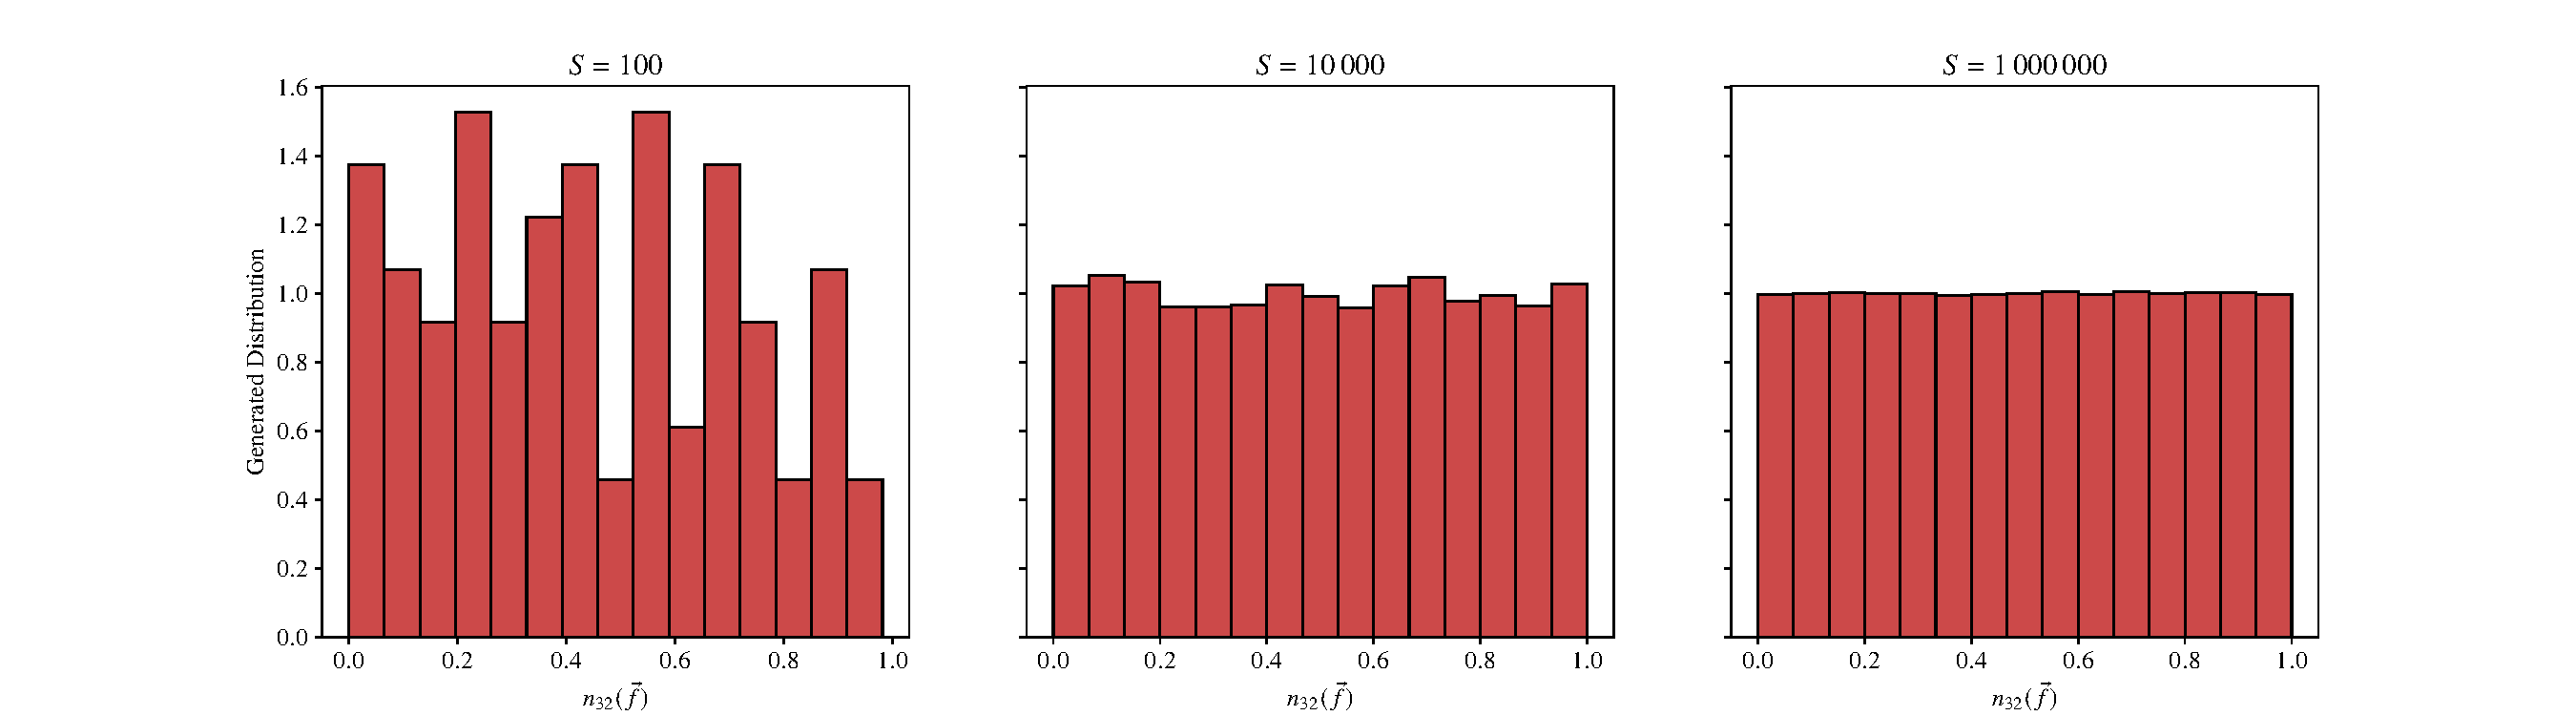
\includegraphics[width=\linewidth]{fair_coin_flips_hist.pdf}
    \caption{Histograms of $n_{32}(\vec f)$ for different number sequences.}
    \label{fig:coin_flip_hist}
\end{figure}
